\tab Urmatorul pas , dupa crearea fisierelor, este sa facem primul commit utilizind : 
\textbf{git add .} - adauga toate fisierele cu continut text si nu numai ce se afla in directoare , pentru a fi inregistrate (caracterul punct == toate)\\
\textbf{git commit -m} - salveaza toate modificarile aduse la fisierele noastre\\
\textbf{git push origin master} - incarca toate modificarile pe \textbf{http://github.com}\\

\begin{figure}[h]
\centering
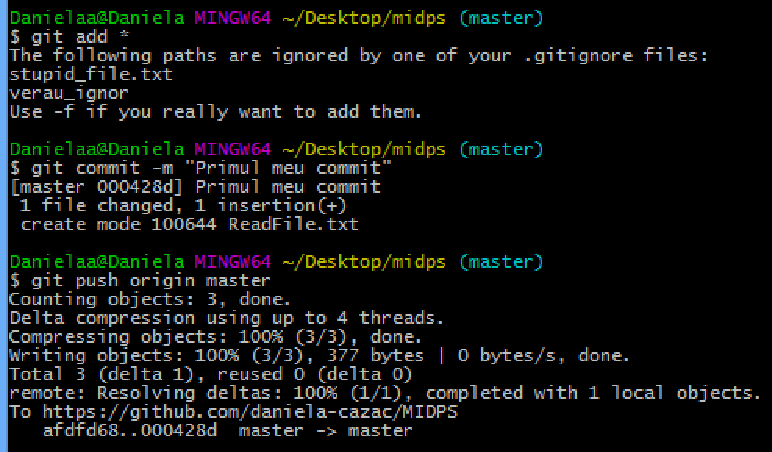
\includegraphics[scale=1]{FirstComit.pdf}
\end{figure}

\clearpage
